%ullright document template
%default a4 one-sided article page setup
\documentclass[article, a4paper, oneside, 11pt]{memoir}

%the following three commands are necessary when using pdflatex
%(set input/output encoding)
\usepackage[utf8]{inputenc}
\usepackage[T1]{fontenc}
\usepackage{helvet}

%use sans serife font for body 
\renewcommand*\familydefault{\sfdefault}


%but with more tech-doc like margins
\setlrmarginsandblock{2.8cm}{2.8cm}{*}
\checkandfixthelayout

%for the german language
\usepackage[ngerman]{babel}

%including pictures
\usepackage{graphicx}
\graphicspath{{./figures/}}

%wrapping text around figures
\usepackage{wrapfig}

%provides symbols for shift, enter, etc.
\usepackage{keystroke}

%url handling
\usepackage{url}

%for code examples
\usepackage{listings}

%elaborate references
\usepackage[ngerman]{varioref}

%enables pdf linking and attributes
\usepackage{hyperref}
\hypersetup{
    colorlinks=true,%
    citecolor=black,%
    filecolor=black,%
    linkcolor=ullblue,%
    urlcolor=ullblue,%
    pdfauthor={ull.at},%
}

%removes page number from frontpage
\pagestyle{empty}

%header and footer images on every page
\usepackage{wallpaper}
\ULCornerWallPaper{1.0}{../../../ullCorePlugin/doc/manual/figures/header}
\LLCornerWallPaper{1.0}{../../../ullCorePlugin/doc/manual/figures/footer}

%Precise figure placement
% \usepackage{float}

%padding for fbox borders
%\setlength\fboxsep{0pt}

%color headlines
\usepackage{color}
\usepackage{titlesec}

\definecolor{ullblue}{rgb}{0.1, 0.42, 0.59}


\titleformat{\chapter}{\color{ullblue}\normalfont\huge\bfseries}{\thechapter}{0.75em}{\huge}

%each chapter on a new page
\let\stdchapter\chapter
\renewcommand*{\chapter}{\clearpage\stdchapter}

%each chapter title starts at the top of the page (reduce top margin)
\titlespacing{\chapter}{0pt}{-3em}{2em}

% Do not indent paragraphes but add newlines
\usepackage{parskip}
\setlength{\parindent}{0cm}
\setlength{\parskip}{2mm}


%memoir recommendation
\clubpenalty=10000
\widowpenalty=10000
\raggedbottom


\hypersetup{
    pdftitle={ullNewsletter Handbuch},%
    pdfsubject={ullright - ullNewsletter}
}

%%%%%%%%%%%%%%%%%%%%%%%%
% Document starts here %
%%%%%%%%%%%%%%%%%%%%%%%%


\begin{document}

\vspace*{3cm}
%move picture left/right
\begin{figure}[htp]
\centering

\includegraphics[width=0.5\textwidth]{softwarebox}
\end{figure}

\vspace{3cm}


{
\huge
\color{ullblue}
ullNewsletter -- Erfolg durch informierte Kunden
}

\vspace{1cm}

Ein Modul der ullright-Plattform -- \href{http://www.ullright.org}{www.ullright.org}

Online ausprobieren unter \href{http://demo.ullright.org}{demo.ullright.org}. 

Zuletzt geändert: 07.12.2011 -- Klemens Ullmann-Marx

\clearpage

\pagestyle{plain}

%number and include in toc up until subsections
\setcounter{secnumdepth}{2}
\setcounter{tocdepth}{2}
\tableofcontents*

\clearpage

\chapter{Überblick}

ullNewsletter ist ein leistungsfähiges Modul der ullright Plattform zum Versand von E-Mail Newslettern.

Hinter einer sehr einfachen Bedienoberfläche arbeitet ein komplexes System um Ihre Newsletter verlässlich und mit größtmöglicher Sicherheit an Ihre Kunden zu versenden.

Die wichtigsten Funktionen:

\begin{itemize}
 \item Personalisierte Newsletter (z.B. mit persönlicher Anrede)
 \item Beliebig viele Verteiler für unterschiedliche Zielgruppen können angelegt werden
 \item Mehrere Layouts können hinterlegt und beim Versand ausgewählt werden
 \item HTML-E-Mails und Grafiken werden unterstützt
 \item Einfache Abmeldung (Unsubscribe)
 \item Automatisierte Behandlung von fehlerhaften Empfänger-Adressen und Out-of-Office Antworten (Bounce-Management)
 \item Online Version zum Ansehen des Newsletters auf Ihrer Website
 \item Tracking zur Kontrolle des Erfolgs Ihrer Kampagne
\end{itemize}

\chapter{Startseite}

Klicken Sie auf "`Newsletter"' um zur Startseite der Newsletter-Verwaltung zu gelangen

Als Modul der ullright Plattform ist die `Startseite` wie üblich aufgebaut (Abbildung \vref{fig:index}):

\begin{figure}[htp]
\centering
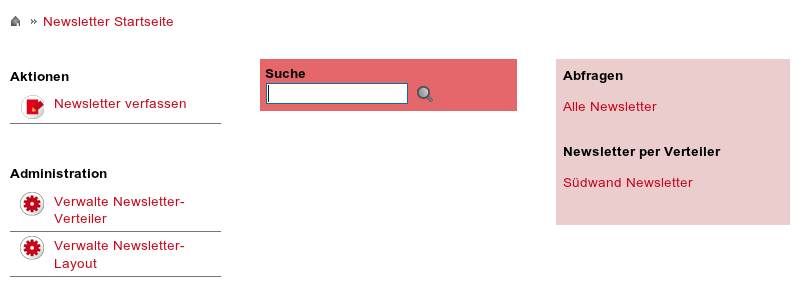
\includegraphics[width=0.9\textwidth]{index}
\caption{Startseite der Newsletter-Verwaltung}
\label{fig:index}
\end{figure}


\section{Newsletter verfassen}

Klicken Sie auf der auf "`Newsletter verfassen"' um einen neuen Newsletter zu erstellen. Alles weitere erfahren Sie im Kapitel \vref{sec:edit}.

\section{Administration - Verwalte Verteiler}

Erstellen und Verwalten der verschiedenen Verteiler. Siehe Kapitel \vref{sec:verteiler}. 

\section{Administration - Verwalte Layouts}

Erstellen und Verwalten von Layouts für Newsletter. Siehe Kapitel \vref{sec:layouts}. 


\section{Suche}

Durchsucht den Betreff der bisher versandten Newsletter.

Geben Sie eine Suchbegriff oder auch nur einen Teil davon in das Suchfeld ein und drücken Sie $\Enter$ oder klicken Sie das Lupen-Symbol an.

\section{Abfragen}

Öffnen Sie eine Liste aller Newsletter, oder wählen Sie eine Liste eines bestimmten Verteilers. Siehe auch Kapitel \vref{sec:list}.



\chapter{Listenansicht}
\label{sec:list}

In der Listenansicht sehen Sie einen Überblick Ihrer Newsletter.

\begin{figure}[htp]
\centering

\includegraphics[width=0.9\textwidth]{list}
\caption{Liste der Newsletter}
\label{fig:list}
\end{figure}

\section{Filtereinstellungen}

Filter schränken die Anzeige der Listenansicht nach verschiedenen Kriterien ein.

Klicken Sie auf das Papierkorbsymbol eines Filters um es zu entfernen.

\section{Aktionsleiste}

In der Aktionsleiste können Sie einen neuen Newsletter verfassen ("`Erstellen"') oder die die Liste nach gewissen Kriterien filtern bzw. durchsuchen.

Das Suchfeld sucht im Betreff der angezeigten Newsletter.

\section{Liste}

In der Liste selbst sehen Sie die wichtigsten Informationen zum Status der einzelnen Newsletter.

\subsection{Bearbeiten}

Klicken Sie auf das Stiftsymbol um einen Newsletter zu bearbeiten. Siehe hierzu auch Kapitel \vref{sec:edit}.

\subsection{Gesamtanzahl Empfänger}

Zeigt Ihnen die Anzahl der Empfänger. Diese Zahl ergibt sich aus der Summe der Abonnenten der jeweils für den Newsletter ausgewählten Verteiler.

\subsection{Versandt}

Zeigt die Anzahl der Newsletter die tatsächlich versandt wurden. Klicken Sie auf die Zahl um eine Liste aller Empfänger zu sehen.

Falls die Zahl kleiner als die Gesamtanzahl der Empfänger ist, gibt es fehlerhafte E-Mailadressen. Klicken Sie in der gleichen Zeile auf die Zahl der unzustellbaren Newsletter um Näheres über die Fehler herauszufinden.

\subsection{Gelesen}

Hier sehen Sie wieviele Ihrer Empfänger den Newsletter gelesen haben. Klicken Sie auf die Zahl um Details anzuzeigen. Siehe dazu Kapitel \vref{sec:tracking}

Bitte beachten Sie, dass es nicht alle E-Mailprogramme erlauben herauszufinden ob ein Empfänger den Newsletter gelesen hat. Daher ist diese Zahl mit Vorsicht zu genießen.

\subsection{Unzustellbar}

Zeigt wieviele Newsletter unzustellbar waren. Klicken Sie auf die Zahl um Details anzusehen. Details dazu finden Sie im Kapitel \vref{sec:undeliverable}



\chapter{Newsletter verfassen}
\label{sec:edit}

Klicken Sie auf der Newletter-Startseite, oder in der Listenansicht auf "`Erstellen"'.

\begin{figure}[htp]
\centering

\includegraphics[width=0.9\textwidth]{edit}
\caption{Newsletter verfassen}
\label{fig:edit}
\end{figure}

\section{Felder}

\subsection{Verteiler}

Wählen Sie einen oder mehrere Verteiler an den Sie den Newletter senden möchten
Verteiler die in der Verwaltung (siehe Kapitel \vref{sec:verteiler}) als Standardverteiler markiert wurden sind bereits ausgewählt.

\subsection{Betreff}

Geben Sie einen Betreff ein.

\subsection{Text}

Den Inhalt Ihres Newsletter geben Sie im Feld "`Text"' ein. Es steht Ihnen eine WYSIWYG-Editor ähnlich wie von Word oder OpenOffice gewohnt zur Verfügung. Sie können also Überschriften, Aufzählunglisten und Schriftformatierungen wählen. Auch das Einfügen von Links und Bildern ist möglich.

Ausführliche Informationen zum Editor erhalten Sie im Kapitel \vref{sec:editor}

Für personalisierte E-Mails können Sie eine Reihe von Platzhaltern verwenden.

Beispiele:
\begin{description}
 % "[" is interpreted -> use \lbrack instead
 % the underscore in ONLINE_LINK is interpreted (!?%&) -> escape with \
 \item[\lbrack FIRST\_NAME\rbrack] Der Vorname des Empfängers
 \item[\lbrack LAST\_NAME\rbrack] Der Nachname des Empfängers
 \item[\lbrack TITLE\rbrack] Der Titel
\end{description}

Beispiel: Hallo [FIRST\_NAME] [LAST\_NAME]!

\subsection{Layout}

Wählen Sie ein Layout aus der Liste. Im Normalfall ist Ihr Standardlayout bereits vor-ausgewählt.

\section{Aktionen}

\subsection{Speichern und ansehen}

Wenn Sie mit dem Verfassen fertig sind, können Sie sich mittels "`Speichern und ansehen"' eine Online-Vorschau ansehen. Aus der Online Vorschau gelangen Sie durch Klick auf das Stift-Icon zurück zum Bearbeitungsmodus.

\subsection{Sende Test-Newsletter an mich}

Des weiteren können SIe mit "`Sende Test-Newsletter an mich"' einen Newsletter an Ihre eigene E-Mailadresse zusenden um die Darstellung im E-Mailprogramm zu überprüfen.

\subsection{Sende Newsletter}

Sind Sie zufrieden senden Sie den Newsletter durch Klick auf "`Sende Newsletter"' ab. Bestätigen dazu die Sicherheitsabfrage.

Sie werden nun zur Listenansicht weitergeleitet und erhalten eine Meldung an wieviele Empfänger der Aufrag zur Sendung des Newsletters entgegengenommen wurde.

Je nach Anzahl der Empfänger kann das Versenden bis zu mehreren Stunden dauern. Sie können jederzeit nachsehen wieviele E-Mails bereits versendet wurden in dem Sie die Listenansicht aktualisieren (Taste $\keystroke{F5}$ im Webbrowser).


\subsection{Zwischenspeichern}

Wählen Sie "`Zwischenspeichern"' um während des Verfassens den bereits eingegebenen Text zu sichern.

\subsection{Speichern und zurück zur Liste}

Wenn Sie den Newsletter noch nicht versenden möchten, oder wenn Sie einen Fehler korrigiert haben gelangen Sie mit "`Speichern und zurück zur Liste"' zurück zur Listenansicht.

Auch wenn Sie den Newsletter bereits losgeschickt haben kann es sinnvoll sein Fehler für die Darstellung im Online-Archiv zu korrigieren.



\chapter{Tracking}
\label{sec:tracking}

ullNewsletter erlaubt Ihnen eine Vielzahl an Information über die Leser Ihres Newsletters herauszufinden.

Bitte beachten Sie, dass es nicht alle E-Mailprogramme erlauben herauszufinden ob ein Empfänger den Newsletter gelesen hat. Daher sind die Zahlen mit Vorsicht zu genießen.

\section{Liste}

Gehen Sie auf die Startseite der Newsletter-Verwaltung und wählen Sie "`Abfragen - Alle Newsletter"'. 

Klicken Sie nun auf die Zahl in der Spalte "`Gelesen"' des gewünschten Newsletters.


\begin{figure}[htp]
\centering
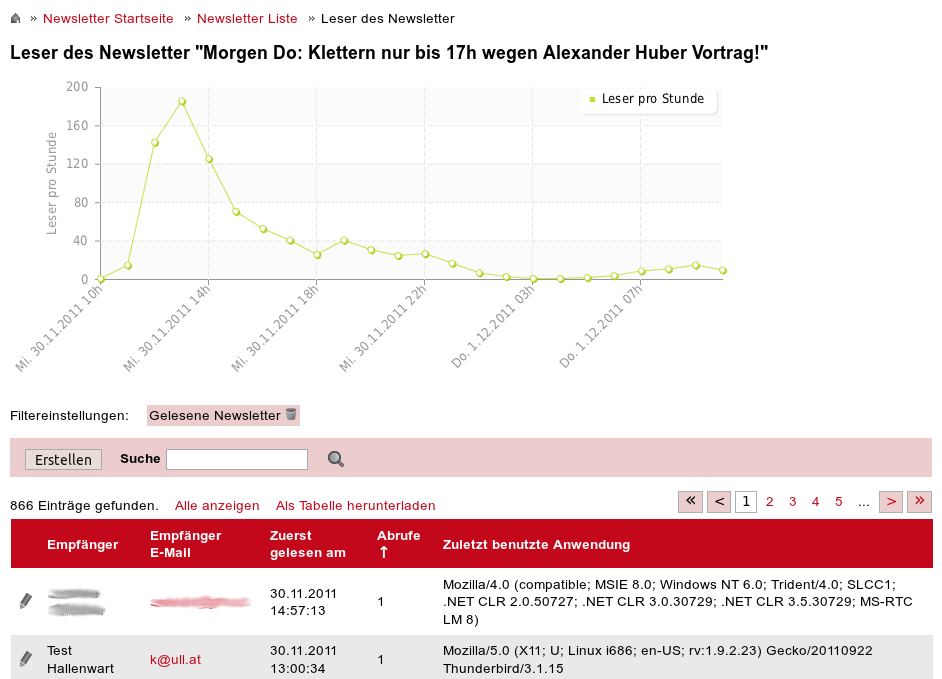
\includegraphics[width=0.9\textwidth]{tracking}
\caption{Tracking}
\label{fig:tracking}
\end{figure}

Zuoberst sehen Sie ein Diagramm, dass den zeitlichen Verlauf der Anzahl Ihrer Leser zeigt.

Danach folgt eine Liste aller Leser Ihres Newsletters. 

Benutzen Sie die Suchfunktion (Durchsucht Name und E-Mail der Empfänger), oder sortieren Sie nach einer der Spalten um mehr über Ihre Leserschaft herauszufinden.

Klicken Sie auf das Stiftsymbol um alle Details anzuzeigen.



\chapter{Unzustellbare Newsletter}
\label{sec:undeliverable}

ullNewsletter bietet eine komfortable, voll-automatisierte Behandlung von fehlerhaften Empfänger-Adressen und Out-of-Office Antworten (Bounce-Management).

Nicht zustellbare Newsletter werden automatisch abgearbeitet und kategorisiert.
Nach einer gewissen Anzahl (Standard: 3) an Fehlern, wird die E-Mailadresse automatisch bereinigt, sodass keine Newsletter mehr an dieses Fehlerhafte E-Mailadresse versendet werden.

Selbstverständlich können Sie einen Liste der unzustellbaren E-Mails und deren Fehlergrund abrufen.

\section{Liste}

Gehen Sie auf die Startseite der Newsletter-Verwaltung und wählen Sie "`Abfragen - Alle Newsletter"'. 

Klicken Sie nun auf die Zahl in der Spalte "`Unzustellbar"' des gewünschten Newsletters.

Sie sehen nun eine Liste aller unzustellbaren Newsletters, neueste Fehlermeldungen oben.

Benutzen Sie die Suchfunktion (Durchsucht Name und E-Mail der Empfänger), oder sortieren Sie nach einer der Spalten um mehr herauszufinden.

Klicken Sie auf das Stiftsymbol um alle Details inklusive der vollständigen Fehlermeldung anzuzeigen.

Nutzen Sie diese Daten um Fehler zu korrigieren, bzw die aktuelle E-Mailadressen Ihrer Empfänger herauszufinden um den maximalen Erfolg Ihrer Kampagnen zu gewährleisten.


\chapter{Abonneten verwalten}

Die ullright Webplattform bietet eine einheitliche und zentrale Benutzerverwaltung. Auch die Abonnenten Ihrer Newsletter sind ganz normale Benutzer.

Folgerichtig erfolgt die Verwaltung der Abonneten hauptsächlich in der Benutzerverwaltung.

Sie finden diese im Adminmenü unter dem Punkt "`Admin"'.

\section{Person hinzufügen (Subscribe)}

Klicken Sie der "`Admin-Startseite"' auf "`Erstelle Benutzer"' und geben Sie die gewünschten Daten ein.

Wählen Sie im Feld "`Newsletter"' die gewünschten Verteiler.

Klicken Sie dann auf "`Speichern und zurück zur Liste"'.


Ist die Person bereits als Benutzer in ullright angelegt benutzen Sie das Suchfeld auf der "`Admin-Startseite"', klicken Sie dann auf das Stiftsymbol, und wählen Sie im Feld "`Newsletter"' die gewünschten Verteiler.


\section{Person von Verteiler abmelden (Unsubscribe)}

Sie haben zwei Möglichkeiten:

\subsection{Person vom Verteiler entfernen}

Benutzen Sie das Suchfeld auf der "`Admin-Startseite"', klicken Sie dann auf das Stiftsymbol der gewünschten Person, und entfernen Sie im Feld "`Newsletter"' die gewünschten Verteiler.

Danach bitte speichern.

\subsection{Benutzer deaktivieren}

Benutzen Sie das Suchfeld auf der "`Admin-Startseite"', klicken Sie dann auf das Stiftsymbol der gewünschten Person, und setzen Sie das Feld "`Status"' auf "`inaktiv"'.

Die Person ist in der ullright Plattform nun komplett deaktiviert.

Danach wählen Sie speichern und zurück zur Liste.



\chapter{Verteiler verwalten}
\label{sec:verteiler}

Legen Sie Verteiler für jede Zielgruppe an. Sie sprechen so jede Interessentengruppe gezielt an und vermeiden Abmeldungen wegen uninteressanten Informationen für Ihre Kunden.

\section{Liste}

Gehen Sie auf die Startseite der Newsletter-Verwaltung und wählen Sie "`Verwalte Newsletter Verteiler"'. Sie gelangen damit zur Listenansicht, wo Sie einen Überblick über Ihre Verteiler sehen.

\begin{figure}[htp]
\centering
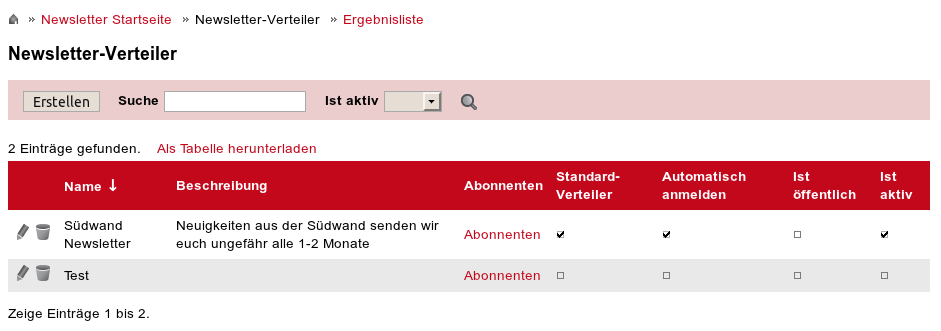
\includegraphics[width=0.9\textwidth]{mailing_lists}
\caption{Liste der Verteiler}
\label{fig:mailing_lists}
\end{figure}

\subsection{Abonnenten}

Klicken Sie in der Zeile des gewünschten Newsletters auf "`Abonnenten"' um eine Liste aller Personen abzurufen die diesen Newsletter abonniert haben.


\section{Erstellen und Bearbeiten}
\label{sec:create-mailing-list}

Wählen Sie "`Erstellen"' um einen neuen Verteiler anzulegen.

Klicken Sie auf das Stiftsymbol des gewünschten Verteilers um ihn zu bearbeiten.

\begin{figure}[htp]
\centering
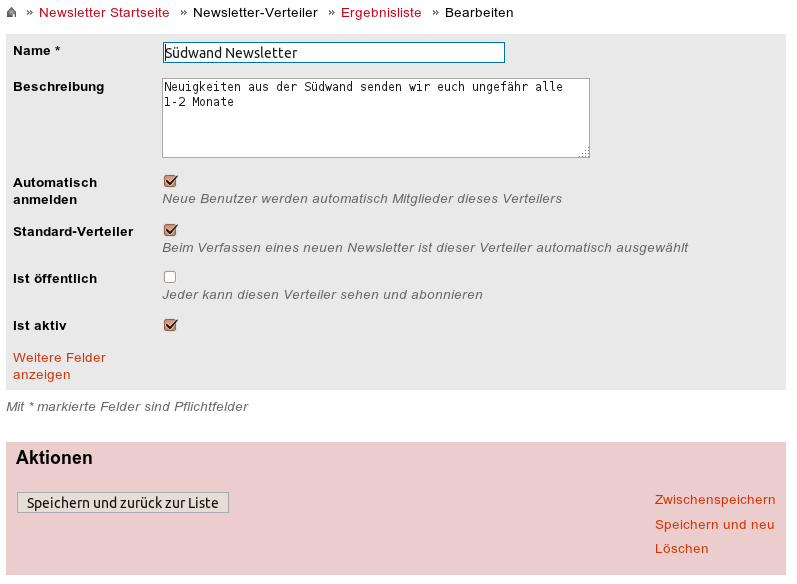
\includegraphics[width=0.9\textwidth]{mailing_lists_edit}
\caption{Verteiler Bearbeitungsmodus}
\label{fig:mailing_lists_edit}
\end{figure}


\subsection{Name}

Geben Sie den Namen für den Verteiler ein.

Beispiel: Produktneuigkeiten für Gemüsehändler

\subsection{Beschreibung}

Beschreiben Sie welche Informationen Ihre Kunden über diesen Verteiler erhalten.

Denken Sie an folgende Punkte:
\begin{itemize}
 \item Zielgruppe
 \item Themen
 \item Anzahl der Newsletter pro Jahr
\end{itemize}

Beispiel:  

Erhalten Sie 4-6 Mal jährlich interessante Produktneuigkeiten und Erfahrungsberichte aus dem Bereich des Gemüsehandels.

\subsection{Automatisch anmelden}

Hier geht es darum ob neu angelegte Benutzer automatisch für den aktuellen Newsletter angemeldet werden.
Dabei ist es egal ob Sie einen Benutzer händisch anlegen oder ob sich der Benutzer selbst auf Ihrer Webseite registriert.

\subsection{Standard-Verteiler}

Wenn Sie dieses Feld anhaken wird beim Verfassen eines neuen Newsletter dieser Verteiler automatisch ausgewählt.

\subsection{Ist öffentlich}

Wenn Sie "`Ist öffentlich"' anhaken kann jeder diesen Verteiler sehen und abonnieren.

\subsection{Ist aktiv}

Damit steuern Sie ob der aktuelle Verteiler aktiv ist. Entfernen Sie das Häkchen wenn Sie diesen Verteiler nicht mehr verwenden möchten.





\chapter{Layouts verwalten}
\label{sec:layouts}

Ein Layout ist eine Art Formatvorlage um Ihren Newslettern ein einheitliches und attraktives Aussehen zu verleihen.

Im Normalfall genügt es einmal ein Layout im Stile Ihrer CI (Corporate Identity) anzulegen.

Sie können beliebig viele Layouts anlegen.


\section{Liste}

Gehen Sie auf die Startseite der Newsletter-Verwaltung und wählen Sie "`Verwalte Newsletter Layouts"'. Sie gelangen damit zur Listenansicht, wo Sie einen Überblick über Ihre Layouts sehen.

\section{Erstellen und Bearbeiten}
\label{sec:create-layout}

Wählen Sie "`Erstellen"' um ein neues Layout anzulegen.

Klicken Sie auf das Stiftsymbol des gewünschten Layouts um es zu bearbeiten.

\subsection{Name}

Geben Sie einen Namen für das neue Layout ein. Beispiel: "`Standard"'

\subsection{HTML-Head}

Der "`head"' Teil des HTML Codes. Hier können Sie z.B. CSS Stylesheet Anweisungen einfügen.

Beispiel:

\begin{lstlisting}
<style type="text/css">
  body {
    font-size 10pt; 
  }
  
  h1 { 
    color: red;
  } 
</style>
\end{lstlisting}

Hinweis: Der "`<head>"' Tag ist nicht erforderlich, er wird automatisch eingefügt.

\subsection{HTML-Body}

Geben Sie hier den HTML-Code für Ihr Layout ein.

Sie können den grafischen WYSIWYG (What you see is what you get) Editor (Siehe Kapitel \vref{sec:editor}) verwenden oder durck Klick auf den Button "`Quellcode"' zum HTML-Code umschalten.

Folgende Platzhalter stehen zur Verfügung:

\begin{description}
 % "[" is interpreted -> use \lbrack instead
 % the underscore in ONLINE_LINK is interpreted (!?%&) -> escape with \
 \item[\lbrack ONLINE\_LINK\rbrack] Fügt den Link zur Online-Version des Newsletters ein ("`Haben Sie Probleme mit der Ansicht des Newsletters klicken Sie hier..."')
 \item[\lbrack CONTENT\rbrack] Platzhalter für den eigentlichen Inhalt des Newsletters
 \item[\lbrack UNSUBSCRIBE\rbrack] Fügt die Unsubscribe-Links zur Abmeldung ein
 \item[\lbrack TRACKING\rbrack] Fügt die Funktionalität für das Tracking ein ("`Wer hat den Newsletter gelesen"')
\end{description}


Ein einfaches Beispiel:

\begin{lstlisting}
<h1>ullright Product News</h1>

<p>[ONLINE_LINK]<p>

<p>[CONTENT]</p>

<p>[UNSUBSCRIBE]</p>
<p>(C) 2011 by ull.at</p>
\end{lstlisting}

\subsection{Ist Standardlayout}

Wenn Sie dieses Feld anhaken wird dieses Layout beim Verfassen eines neuen Newsletter automatisch vor-ausgewählt.


\chapter{Text bearbeiten mit dem "`WYSIWYG"' Editor}
\label{sec:editor}

"`WYSIWYG"' steht für "`What you see is what you get"',  also dass man schon bei der Eingabe sieht wie der Text letztendlich aussehen wird.

Die angezeigten Formatierungs-Möglichkeiten können sich je nach Konfiguration und Editor-Version von Ihrer Installation unterscheiden.

\begin{figure}[htp]
\centering
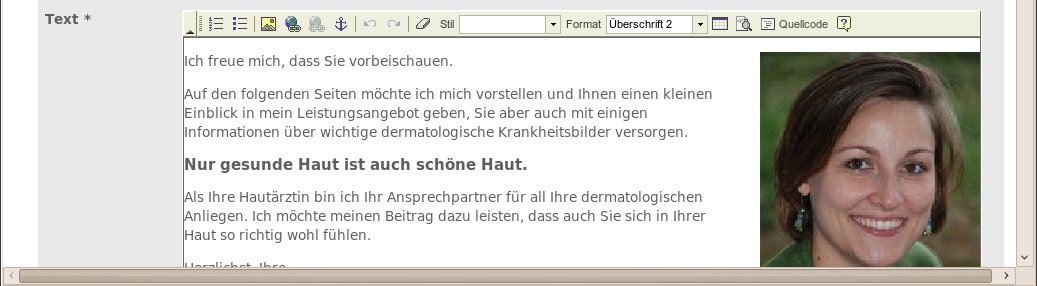
\includegraphics[width=0.9\textwidth]{../../../ullCorePlugin/doc/manual/figures/editor}
\caption{WYSIWYG-Editor}
\label{fig:editor}
\end{figure}

\section{Text schreiben}

Geben Sie wie von anderen Texteditoren gewohnt den Text ein.

Tipp: $\Enter$ erzeugt einen neuen Paragrafen, also einen Textblock mit einer Leerzeile dahinter. Einen einfachen Zeilenumbruch erreichen Sie mit $\Shift + \Enter$.

\section{Text formatieren}

Markieren Sie den gewünschten Text und wählen Sie aus der Editor-Menüleiste die gewünschte Auszeichnung.

Bitte beachten Sie, dass die von uns ausgewählten
Formatierungsmöglichkeiten nach semantischen Gesichtspunkten ausgewählt
wurden. Sie finden also nur „logische“ Auszeichnungen wie zum Beispiel
„wichtig“ oder „Überschrift“, und keine rein optischen
Formatierungsmöglichkeiten wie Farben oder Schriftgrößen. Somit werden
saubere und zukunftssichere Texte gewährleistet. (Stichwort "`semantic
Web"')

Die wichtigsten Formatierungen (von links nach rechts):

\begin{itemize}
\item Nummerierte Liste
\item Liste mit Aufzählungszeichen
\item Stile: "`Important"' -- also "`Wichtig"' wird fett angezeigt
\item Format: "`Überschrift"'
\end{itemize}


\section{Bild einfügen}

\begin{itemize}
\item Setzten Sie den Cursor an die gewünschte Stelle im Text
\item Klicken Sie auf das Bildsymbol 
\includegraphics[height=5mm]{../../../ullCorePlugin/doc/manual/figures/image_icon}
\item Wählen Sie "`Server durchsuchen"'
\item Wählen oder erstellen Sie gegebenenfalls einen neuen Ordner um eine ordentliche Struktur Ihrer Daten zu gewährleisten
\item Wenn Sie ein neues Bild hochladen möchten klicken Sie auf "`Durchsuchen"' und wählen Sie eine Bilddatei von Ihrem Computer aus.
\item Vergessen Sie nicht danach auf "`Upload"' zu klicken
\item Wählen Sie nun ein Bild aus der Liste durch anklicken.
\item Klicken Sie auf "`OK"'
\end{itemize}

\section{Bildeigenschaften ändern}

Klicken Sie mit der rechten Maustaste auf das Bild und wählen Sie "`Bildeigenschaften"'.

Im folgenden werden die wichtigsten Eigenschaften erklärt:

\subsection{Reiter "`Bild-Info"'}

\begin{itemize}
\item Breite / Höhe - Wählen Sie die gewünschte Größe des Bildes in Pixel. Bitte beachten Sie, dass Bilder bereits vor dem Hochladen mit einem Grafikprogramm auf die endgültige Größe skaliert werden sollten
\item Ausrichtung - Wählen Sie "`Links"' oder "`Rechts"' wenn der Text das Bild umfließen soll.
\end{itemize}

\subsection{Reiter "`Erweitert"'}

Wenn Sie das Bild vom Text umfließen lassen ist häufig auf gewissen Seiten des Bildes ein Abstand erwünscht.
Dieser Abstand kann im Feld "`Style"' angegeben werden. Beispiel für einen Abstand links und unten: "`margin-left: 1.5em; margin-bottom: 1.5em;"'


\section{Link erstellen}

Normale Webadressen und E-Mailadressen werden in der normalen Ansicht für die Besucher der Webseite automatisch verlinkt.

Beispiele:

\begin{itemize}
\item www.ullright.org
\item http://ull.at
\item office@ull.at
\end{itemize}

Möchten Sie hingegen gewisse Wörter im Text verlinken markieren Sie die Wörter und klicken Sie auf das Linksymbol 
\includegraphics[height=5mm]{../../../ullCorePlugin/doc/manual/figures/link_icon} (blau-grüne Erdkugel).

\subsection{Link zu einer Internetadresse (URL)}
Geben Sie bei "`URL"' die gewünschte Adresse ein. Beispiel: \url{http://www.ullright.org}

Bei Links zu Internetseiten empfiehlt sich die Seite in einem neuen Browserfenster zu öffnen. Wählen Sie hierzu im Reiter "`Zielseite"' "`Neues Fenster (\_blank)"'.

Zusätzlich empfehlen wir einen solchen Link durch das Symbol für "`Externe Seite"' zu kennzeichen. Schreiben Sie dazu im Reiter "`Erweitert"' die Anweisung "`link\_external"' in das Feld "`Stylesheet Klasse"'.

\subsection{Link zu einer anderen CMS-Seite}

Öffnen Sie die Zielseite in einem neuen Browsertab oder -fenster und kopieren Sie die URL aus der Adressleiste.

Beispiel: \url{http://www.ull.at/ullCms/show/kontakt}

Geben Sie nun bei "`URL"' die gekürzte Adresse startend mit den Schrägstrich nach dem Domänennamen ein.

Beispiel: \url{/ullCms/show/kontakt}

\subsection{E-Mail Link}

Wählen Sie bei "`Link-Typ"' E-Mail und geben Sie die gewünschte E-Mailadresse ein.



\section{Datei hochladen}
\label{sec:upload_file}

Das Hochladen einer Datei funktioniert wie eine Mischung aus Link- und Bildeinfügen.

\begin{itemize}
\item Markieren Sie die Wörter die mit der Datei verlinkt werden sollen
\item Klicken Sie auf das Linksymbol 
\includegraphics[height=5mm]{../../../ullCorePlugin/doc/manual/figures/link_icon}
\item Wählen Sie „Server durchsuchen“
\item Wählen oder erstellen Sie gegebenenfalls einen neuen Ordner um eine ordentliche Struktur Ihrer Daten zu gewährleisten
\item Wenn Sie eine neue Datei hochladen möchten klicken Sie auf "`Durchsuchen"' und wählen Sie eine Datei von Ihrem Computer aus
\item Vergessen Sie nicht danach auf "`Upload"' zu klicken
\item Wählen Sie nun die Datei aus der Liste durch anklicken
\item Klicken Sie auf "`OK"'
\end{itemize}


\section{Tip für PDF-Dateien}

Auf vielen PCs wird bei einem Klick auf den Link zu einer PDF-Datei das PDF direkt im Browserfenster geöffnet. Besuchern passiert es dann häufig, dass sie nach dem Lesen das Fenster oder Tab einfach schließen, und somit auch Ihre Website verlassen.

Um diesem unerwünschten Verhalten vorzubeugen empfiehlt sich ein PDF in einem Pop-up Fenster zu öffnen:

\begin{itemize}
\item Verlinken Sie eine PDF-Datei wie im Kapitel \vref{sec:upload_file} beschrieben
\item Klicken Sie mit der rechten Maustaste auf den Link zur PDF-Datei und wählen Sie "`Link editieren"'
\item Im Reiter "`Zielseite"' wählen Sie nun "`Pop-up Fenster"'
\item Haken Sie die Felder "`Vergrößerbar"', "`Adress-Leiste"', "`Menüleiste"' und "`Rollbalken"' an.
\item Schließen Sie den Vorgang mit "`OK"' ab.
\end{itemize}


\chapter{Quellenangaben}

Danke an folgende ull.at Kunden, die Screenshots ihrer Webseiten zur Verfügung stellten:

\begin{itemize}
\item Dr. Tamara Meissnitzer - \href{http://www.hautarzt.md}{www.hautarzt.md}
\item Kletterzentrum Südwand - \href{http://http://www.kletterzentrum-suedwand.at/}{http://www.kletterzentrum-suedwand.at/}
\item ullright Demoseite - \href{http://demo.ullright.org}{demo.ullright.org}
\end{itemize}

\end{document}